\documentclass[11pt,preprint, authoryear]{elsarticle}

\usepackage{lmodern}
%%%% My spacing
\usepackage{setspace}
\setstretch{1.2}
\DeclareMathSizes{12}{14}{10}{10}

% Wrap around which gives all figures included the [H] command, or places it "here". This can be tedious to code in Rmarkdown.
\usepackage{float}
\let\origfigure\figure
\let\endorigfigure\endfigure
\renewenvironment{figure}[1][2] {
    \expandafter\origfigure\expandafter[H]
} {
    \endorigfigure
}

\let\origtable\table
\let\endorigtable\endtable
\renewenvironment{table}[1][2] {
    \expandafter\origtable\expandafter[H]
} {
    \endorigtable
}


\usepackage{ifxetex,ifluatex}
\usepackage{fixltx2e} % provides \textsubscript
\ifnum 0\ifxetex 1\fi\ifluatex 1\fi=0 % if pdftex
  \usepackage[T1]{fontenc}
  \usepackage[utf8]{inputenc}
\else % if luatex or xelatex
  \ifxetex
    \usepackage{mathspec}
    \usepackage{xltxtra,xunicode}
  \else
    \usepackage{fontspec}
  \fi
  \defaultfontfeatures{Mapping=tex-text,Scale=MatchLowercase}
  \newcommand{\euro}{€}
\fi

\usepackage{amssymb, amsmath, amsthm, amsfonts}

\def\bibsection{\section*{References}} %%% Make "References" appear before bibliography


\usepackage[round]{natbib}

\usepackage{longtable}
\usepackage[margin=2.3cm,bottom=2cm,top=2.5cm, includefoot]{geometry}
\usepackage{fancyhdr}
\usepackage[bottom, hang, flushmargin]{footmisc}
\usepackage{graphicx}
\numberwithin{equation}{section}
\numberwithin{figure}{section}
\numberwithin{table}{section}
\setlength{\parindent}{0cm}
\setlength{\parskip}{1.3ex plus 0.5ex minus 0.3ex}
\usepackage{textcomp}
\renewcommand{\headrulewidth}{0.2pt}
\renewcommand{\footrulewidth}{0.3pt}

\usepackage{array}
\newcolumntype{x}[1]{>{\centering\arraybackslash\hspace{0pt}}p{#1}}

%%%%  Remove the "preprint submitted to" part. Don't worry about this either, it just looks better without it:
\makeatletter
\def\ps@pprintTitle{%
  \let\@oddhead\@empty
  \let\@evenhead\@empty
  \let\@oddfoot\@empty
  \let\@evenfoot\@oddfoot
}
\makeatother

 \def\tightlist{} % This allows for subbullets!

\usepackage{hyperref}
\hypersetup{breaklinks=true,
            bookmarks=true,
            colorlinks=true,
            citecolor=blue,
            urlcolor=blue,
            linkcolor=blue,
            pdfborder={0 0 0}}


% The following packages allow huxtable to work:
\usepackage{siunitx}
\usepackage{multirow}
\usepackage{hhline}
\usepackage{calc}
\usepackage{tabularx}
\usepackage{booktabs}
\usepackage{caption}


\newenvironment{columns}[1][]{}{}

\newenvironment{column}[1]{\begin{minipage}{#1}\ignorespaces}{%
\end{minipage}
\ifhmode\unskip\fi
\aftergroup\useignorespacesandallpars}

\def\useignorespacesandallpars#1\ignorespaces\fi{%
#1\fi\ignorespacesandallpars}

\makeatletter
\def\ignorespacesandallpars{%
  \@ifnextchar\par
    {\expandafter\ignorespacesandallpars\@gobble}%
    {}%
}
\makeatother

\newlength{\cslhangindent}
\setlength{\cslhangindent}{1.5em}
\newenvironment{CSLReferences}%
  {\setlength{\parindent}{0pt}%
  \everypar{\setlength{\hangindent}{\cslhangindent}}\ignorespaces}%
  {\par}


\urlstyle{same}  % don't use monospace font for urls
\setlength{\parindent}{0pt}
\setlength{\parskip}{6pt plus 2pt minus 1pt}
\setlength{\emergencystretch}{3em}  % prevent overfull lines
\setcounter{secnumdepth}{5}

%%% Use protect on footnotes to avoid problems with footnotes in titles
\let\rmarkdownfootnote\footnote%
\def\footnote{\protect\rmarkdownfootnote}
\IfFileExists{upquote.sty}{\usepackage{upquote}}{}

%%% Include extra packages specified by user
\usepackage{array}
\usepackage{caption}
\usepackage{graphicx}
\usepackage{siunitx}
\usepackage[normalem]{ulem}
\usepackage{colortbl}
\usepackage{multirow}
\usepackage{hhline}
\usepackage{calc}
\usepackage{tabularx}
\usepackage{threeparttable}
\usepackage{wrapfig}
\usepackage{adjustbox}
\usepackage{hyperref}

%%% Hard setting column skips for reports - this ensures greater consistency and control over the length settings in the document.
%% page layout
%% paragraphs
\setlength{\baselineskip}{12pt plus 0pt minus 0pt}
\setlength{\parskip}{12pt plus 0pt minus 0pt}
\setlength{\parindent}{0pt plus 0pt minus 0pt}
%% floats
\setlength{\floatsep}{12pt plus 0 pt minus 0pt}
\setlength{\textfloatsep}{20pt plus 0pt minus 0pt}
\setlength{\intextsep}{14pt plus 0pt minus 0pt}
\setlength{\dbltextfloatsep}{20pt plus 0pt minus 0pt}
\setlength{\dblfloatsep}{14pt plus 0pt minus 0pt}
%% maths
\setlength{\abovedisplayskip}{12pt plus 0pt minus 0pt}
\setlength{\belowdisplayskip}{12pt plus 0pt minus 0pt}
%% lists
\setlength{\topsep}{10pt plus 0pt minus 0pt}
\setlength{\partopsep}{3pt plus 0pt minus 0pt}
\setlength{\itemsep}{5pt plus 0pt minus 0pt}
\setlength{\labelsep}{8mm plus 0mm minus 0mm}
\setlength{\parsep}{\the\parskip}
\setlength{\listparindent}{\the\parindent}
%% verbatim
\setlength{\fboxsep}{5pt plus 0pt minus 0pt}



\begin{document}



%titlepage
\thispagestyle{empty}
\begin{center}
\begin{minipage}{0.75\linewidth}
    \centering
%Entry1
    {\uppercase{\huge Real Exchange Rate Behaviour: A Replication and
Robustness Check\par}}
    \vspace{2cm}
%Author's name
    {\LARGE Cassandra Pengelly \textbar{} 20346212\par}
    \vspace{1cm}
%University logo
\begin{center}
    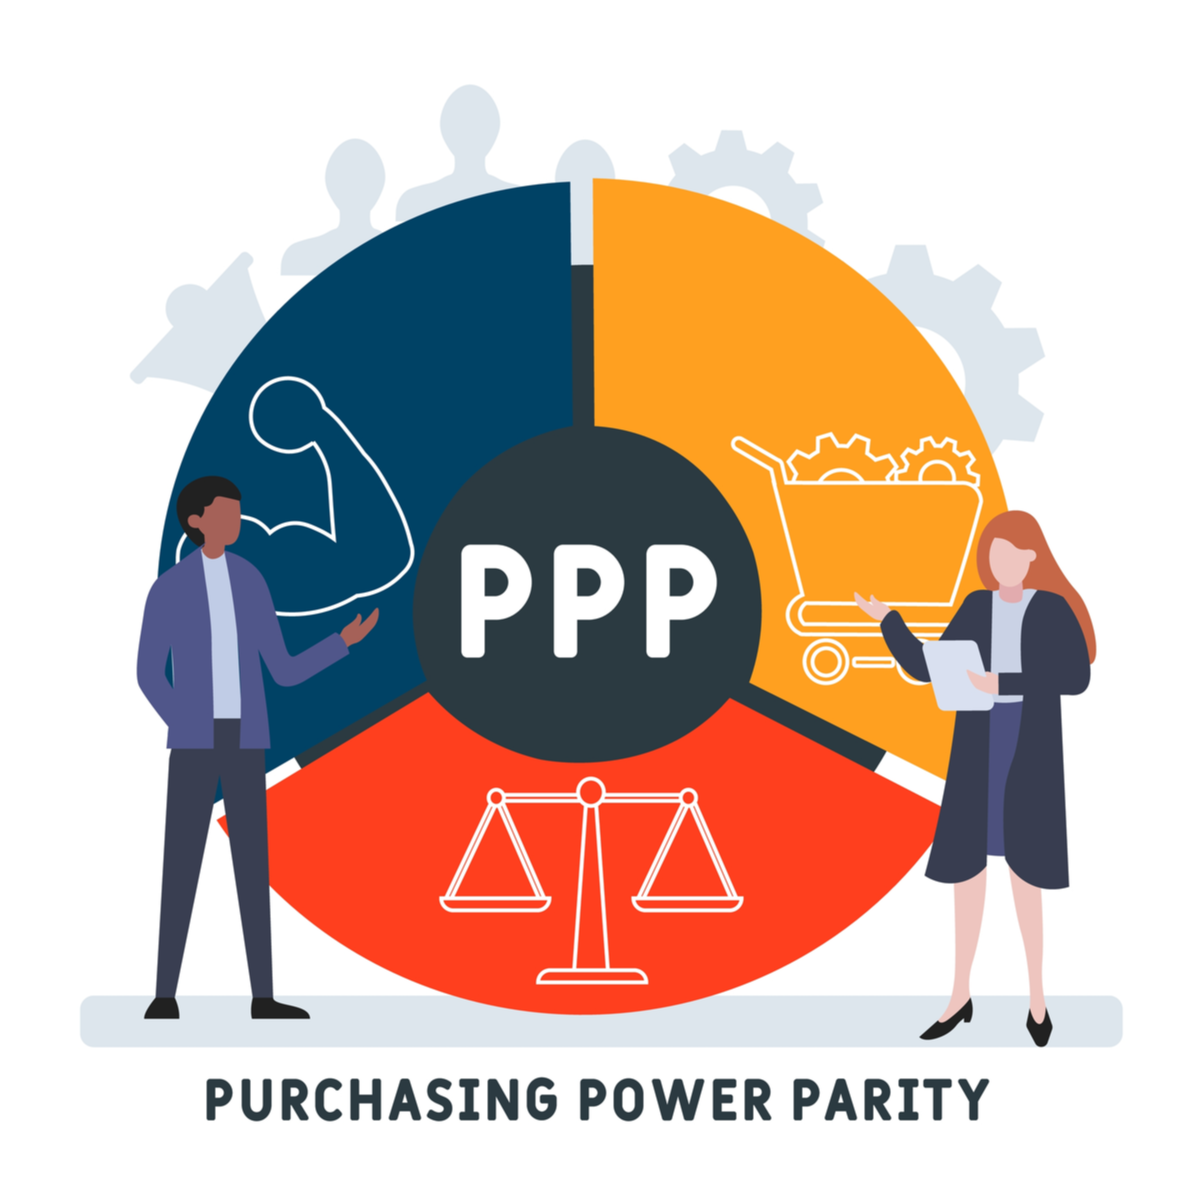
\includegraphics[width=0.5\linewidth]{Tex/Logo.png}
\end{center}
\vspace{1cm}
%Supervisor's Details
\begin{center}
    {\Large Econometrics 871: Time Series Project\par}
    \vspace{1cm}
%Degree
    {\large \par}
    \vspace{1cm}
%Institution
    {\large \par}
    \vspace{1cm}
%Date
    {\large }
%More
    {\normalsize }
%More
    {\normalsize }
\end{center}
\end{minipage}
\end{center}
\clearpage


\begin{frontmatter}  %

\title{}

% Set to FALSE if wanting to remove title (for submission)


\vspace{1cm}





\vspace{0.5cm}

\end{frontmatter}


\renewcommand{\contentsname}{Table of Contents}
{\tableofcontents}

%________________________
% Header and Footers
%%%%%%%%%%%%%%%%%%%%%%%%%%%%%%%%%
\pagestyle{fancy}
\chead{}
\rhead{}
\lfoot{}
\rfoot{\footnotesize Page \thepage}
\lhead{}
%\rfoot{\footnotesize Page \thepage } % "e.g. Page 2"
\cfoot{}

%\setlength\headheight{30pt}
%%%%%%%%%%%%%%%%%%%%%%%%%%%%%%%%%
%________________________

\headsep 35pt % So that header does not go over title




\hypertarget{introduction}{%
\section{\texorpdfstring{Introduction
\label{Introduction}}{Introduction }}\label{introduction}}

How do we compare living standards and economic productivity between
countries? This is one of the questions that macroeconomics attempts to
answers and a number of tools have been developed within the field to
this end. One of these tools is the Purchasing Power Parity (PPP)
theory, which uses a basket of goods to compare the currencies of
different countries. This theory has been widely tested using data, and
the results have been divisive and somewhat puzzling.@puz.

In this essay, I replicate\footnote{More accurately, try my best to
  replicate} the paper ``Real Exchange Rate Behaviour: Evidence from
Black Markets'' by \protect\hyperlink{ref-Kul}{Luintel}
(\protect\hyperlink{ref-Kul}{2000}), which tests the PPP hypothesis. I
include some other tests in addition to those in the paper as a
robustness check on the results.

This essay\footnote{This essay was written in R using the package by
  \protect\hyperlink{ref-Texevier}{Katzke}
  (\protect\hyperlink{ref-Texevier}{2017})} is organised as follows.
Section \ref{Context} contextualises Luintel's paper and discusses the
robustness checks. Section \ref{Data} discusses the data and reports the
results of the Wald-Wolfowitz tests. Section \ref{Unit} deals with the
unit root tests. Section \ref{Var} reports the results of the variance
ratio test and section \ref{Struc} presents the structural break
tests.The code for this replication can be found on Github
\href{https://github.com/cass-code/metrics.git}{here:}.

\hypertarget{context-and-evaluation}{%
\section{\texorpdfstring{Context and Evaluation
\label{Context}}{Context and Evaluation }}\label{context-and-evaluation}}

provide a brief section that outlines the context and questions of the
replicated study: The first part should outline what the authors do, how
they motivate the question as of economic interest and/or importance,
how they motivate their methods and how they argue that their
contribution is novel

The second part can be a critical evaluation of their approach and
choices which leads to your choices of robustness checks/extensions

\protect\hyperlink{ref-Kul}{Luintel} (\protect\hyperlink{ref-Kul}{2000})
investigates whether the PPP hypothesis holds empirically. To test this
theory, \protect\hyperlink{ref-Kul}{Luintel}
(\protect\hyperlink{ref-Kul}{2000}) uses monthly black market real
exchange rates (in terms of the US dollar) from eight developing Asian
countries: India, Sri Lanka, Myanmar, Malaysia, Pakistan, Philippines,
Taiwan and Thailand. The paper finds that

The behaviour of real exchange rates (relative to the US dollar) is
examined using monthly from the black markets for foreign exchange of
eight Asian developing countries. The data The black market real
exchange rates do not show excess volatility during the recent float
contrast to the results reported elsewhere. Unit root tests in
heterogeneous panels and variance confirm their stationarity. Thus, we
find support for PPP but not for the `survivorship' Rogoff, 1995). There
is little evidence of segmented trends. Issues raised by Rogoff (1996)
would hold across countries with differing growth experience-and Lothian
and Taylor whether the degree of relative price volatility may bias
results in favour of mean reverting rates -are addressed. Copyright ©
2000 John Wiley \&

Over the past decade, the purchasing-power parity (PPP) puzzle has taken
two forms. Its early form arose from early tests of unit roots in real
exchange rates, which failed to reject the null hypothesis, thus casting
doubts on the long-term PPP hypothesis of real exchange rates' mean
reversion. Following the development of more powerful tests that
resulted in rejections of unit roots, the PPP-puzzle re-surfaced in the
form of surprisingly slow rates of convergence of real exchange rates to
their long-run means. Rogoff (1996) expressed this puzzle in terms of
the estimated ``half-life'' of real exchange rate shocks being 3 to 5
years. Recent research has attempted to solve that second form of the
puzzle by adopting non-linear stochastic models of real exchange rates.
Despite this introduction of non-linearities, the literature has
continued to focus on the notion of ``half-life'' as a measure of
persistence.

The theory of purchasing power parity (PPP) is one of the most widely
tested economics. The overall findings can be summarized as follows.
Studies based data wholly reject PPP.1 Rogoff (1996, p.~644) calls this
set of evidence `the abject law of one price. Time-series studies based
on aggregate price indices for also largely reject PPP and suggest that
the real exchange rate behaves as random walk hypothesis implies that
shocks to the real exchange rate are persistent is no tendency for PPP
to hold in the short run or in the long run. Rogoff summarizes this set
of findings as 'something of an embarrassment' to the argues that every
`reasonable' theoretical model suggests a mean reverting real the long
run.3

The behaviour of real exchange rates (relative to the US dollar) is
examined using monthly from the black markets for foreign exchange of
eight Asian developing countries. The data The black market real
exchange rates do not show excess volatility during the recent float
contrast to the results reported elsewhere. Unit root tests in
heterogeneous panels and variance confirm their stationarity. Thus, we
find support for PPP but not for the `survivorship' Rogoff, 1995). There
is little evidence of segmented trends. Issues raised by Rogoff (1996)
would hold across countries with differing growth experience-and Lothian
and Taylor whether the degree of relative price volatility may bias
results in favour of mean reverting rates -are addressed. Copyright ©
2000 John Wiley \& Sons, Ltd.~1. INTRODUCTION

\hypertarget{data}{%
\section{\texorpdfstring{Data \label{Data}}{Data }}\label{data}}

The data used for the analysis is a series on black market nominal
exchange rates and consumer price indices (CPI) for 8 developing Asian
countries, namely: India, Sri Lanka, Myanmar, Malaysia, Pakistan,
Philippines, Taiwan and Thailand. I take a subset of these countries by
excluding Taiwan\footnote{I excluded Taiwan because there is some data
  missing from the set and I don't know how to adjust an unbalanced
  panel. However, it is also interesting to test if the results hold
  when taking a subset} from the analysis.
\protect\hyperlink{ref-Kul}{Luintel} (\protect\hyperlink{ref-Kul}{2000})
sources data from various issues of \emph{Pick's Currency Year Book} and
\emph{World Currency Year Book}. The data used for Luintel's paper is
accessible through the Journal of Applied Econometrics archive, which is
where I attained my data. The sample period runs for 31 periods from
January 1958 to June 1989. This sample period is split into two parts:
Bretton Woods and after Bretton Woods (also referred to as pre-float
period and the float period).

The nominal exchange rates are units currencies per unit of US dollar.
There were two mistakes in the nominal exchange rate datasets: for
Myanmar November 1974, there was a value of 1.45, which I replaced with
16.5 (based on interpolation). And for the Philippines in September
1975, there was a value of 0.7 with which I replaced with 7.7 (based on
interpolation).\footnote{I discovered these mistakes when there was a
  dramatic difference in my plots of the real exchange rates and
  Luintel's plots.} Luintel sources the CPI figures from issues of
International Financial Statistics (which are included in Luintel's
dataset available in the JAE data archives).

To calculate the real exchange rates, I follow the lead of
\protect\hyperlink{ref-Kul}{Luintel} (\protect\hyperlink{ref-Kul}{2000})
and apply the following formula to the nominal exchange rates:

\[
rex = log(Nominal Exchange Rate) - log(CPI) + log(United States CPI)
\]

I plot the real exchange rate series below in \ref{Figure1}. The plots
below match those of \protect\hyperlink{ref-Kul}{Luintel}
(\protect\hyperlink{ref-Kul}{2000: 166}) and indicate that the real
exchange rates are trending. Additionally, the graphs show that the
black market exchange rates are somewhat volatile. As expected, we see
that after the first oil shock of 1973 the currencies appreciated and
then slowly reverted. The plots suggest that the trends are segmented. I
test this hypothesis using formal tests, reported below the plots in
\ref{Figure3}.

\begin{center}\includegraphics{20346212_files/figure-latex/Figure1-1} \end{center}
\begin{figure}[H]

{\centering \includegraphics{20346212_files/figure-latex/Figure2-1} 

}

\caption{Plot of Real Exchange Rates over Time\label{Figure1}}\label{fig:Figure2}
\end{figure}

\begin{table}[H]
\centering
\caption{Wald-Wolfowitz tests \label{tab1}} 
\begin{tabular}{lrrrrrrr}
  \hline
Test/Country & India & SriLanka & Malaysia & Myanmar & Pakistan & Philippines & Thailand \\ 
  \hline
Wald-Wolfowitz & -16.07 & -18.54 & -17.10 & -18.23 & -16.27 & -17.10 & -15.96 \\ 
   \hline
\end{tabular}
\end{table}

\hypertarget{unit-root-tests}{%
\section{\texorpdfstring{Unit Root Tests
\label{Unit}}{Unit Root Tests }}\label{unit-root-tests}}

First, I employed the Augmented Dickey-Fuller test for the individual
exchange rates to see whether there was a unit root present. The test
results show

\begingroup\fontsize{11pt}{12pt}\selectfont
\begin{longtable}{lrrr}
\caption{Augmented Dickey-Fuller Tests} \\ 
  \toprule
Countries & Full Sample & Bretton Woods (1958:1-1973:3) & Post-Bretton Woods (1973:4-1989:6) \\ 
  \hline 
\endhead 
\hline 
{\footnotesize Continued on next page} 
\endfoot 
\endlastfoot 
 \midrule
India (Rupee) & -2.70 & -2.07 & -3.66 \\ 
  Sri Lanka (Rupee) & -3.22 & -2.11 & -2.44 \\ 
  Malaysia (Ringgit) & -1.47 & -2.16 & -3.77 \\ 
  Myanmar (Kyat) & -1.53 & -1.71 & -0.16 \\ 
  Pakistan (Rupee) & -3.35 & -2.97 & -5.91 \\ 
  Phillipines (Peso) & -3.09 & -2.07 & -3.38 \\ 
  Thailand (Baht) & -2.44 & -3.36 & -3.93 \\ 
   \bottomrule
\end{longtable}
\endgroup

\hypertarget{panel-unit-root-tests}{%
\subsection{Panel Unit Root Tests}\label{panel-unit-root-tests}}

As noted by \protect\hyperlink{ref-pes}{Breitung \& Pesaran}
(\protect\hyperlink{ref-pes}{2005: 18}), when using country data for
macroeconomic applications, there are often time series contemporaneous
correlations, which is a relevant concern for testing the PPP
hypothesis. There may be unobserved common factors or spatial spillover
effects, which need to be accounted for in the unit root test. Modelling
cross section dependence in panel data sets is still an emerging field,
but \protect\hyperlink{ref-im}{Pasaran, Im \& Shin}
(\protect\hyperlink{ref-im}{1997}) suggest that the appropriate test
statistic is the T-bar test based on cross-sectional demeaned
regressions. This is the

The first unit root test I employ is the Im-Pesaran-Shin t-bar test to
replicate \protect\hyperlink{ref-Kul}{Luintel}
(\protect\hyperlink{ref-Kul}{2000}) test. The results below show that
the null hypothesis (there exists a unit root)

\begingroup\fontsize{12pt}{13pt}\selectfont
\begin{longtable}{lrll}
\caption{IPS Panel Unit Root Tests (Tbar)} \\ 
  \toprule
Test & T-statistic & Trend & Outcome \\ 
  \hline 
\endhead 
\hline 
{\footnotesize Continued on next page} 
\endfoot 
\endlastfoot 
 \midrule
IPS & -2.97 & Yes & Reject H0 \\ 
  IPS & -2.56 & No & Reject H0 \\ 
   \bottomrule
\end{longtable}
\endgroup

I then tests for unit roots using LLL test (I used the package by
\protect\hyperlink{ref-plm}{Millo} (\protect\hyperlink{ref-plm}{2017})
for this).

\hypertarget{variance-ratio-test}{%
\section{\texorpdfstring{Variance Ratio Test
\label{Var}}{Variance Ratio Test }}\label{variance-ratio-test}}

The following table shows results of the Variance Ratio test for the
full sample for up to 20 months. The results of the variance ratio test
for the Bretton Woods period and post Bretton Woods period (for up to 20
months\footnote{The results for 190 months is available upon request; it
  has been omitted purely to save space}) can be found in the Appendix
(\ref{A})

\begingroup\fontsize{12pt}{13pt}\selectfont
\begin{longtable}{lrrrrrrr}
\caption{Variance Ratio Test for Full Sample Up to month 20} \\ 
  \toprule
Months & India & SriLanka & Malaysia & Myanmar & Pakistan & Philippines & Thailand \\ 
  \hline 
\endhead 
\hline 
{\footnotesize Continued on next page} 
\endfoot 
\endlastfoot 
 \midrule
1 & 1.00 & 1.00 & 1.00 & 1.00 & 1.00 & 1.00 & 1.00 \\ 
  se & 0.10 & 0.10 & 0.10 & 0.10 & 0.10 & 0.10 & 0.10 \\ 
  2 & 1.00 & 0.95 & 0.79 & 1.04 & 0.91 & 0.91 & 0.74 \\ 
  se & 0.10 & 0.10 & 0.10 & 0.10 & 0.10 & 0.10 & 0.10 \\ 
  3 & 1.02 & 0.86 & 0.79 & 1.05 & 0.81 & 0.86 & 0.68 \\ 
  se & 0.10 & 0.10 & 0.10 & 0.10 & 0.10 & 0.10 & 0.10 \\ 
  4 & 1.01 & 0.87 & 0.75 & 1.00 & 0.71 & 0.82 & 0.58 \\ 
  se & 0.10 & 0.10 & 0.10 & 0.10 & 0.10 & 0.10 & 0.10 \\ 
  5 & 0.95 & 0.89 & 0.73 & 0.98 & 0.65 & 0.80 & 0.52 \\ 
  se & 0.10 & 0.10 & 0.10 & 0.10 & 0.10 & 0.10 & 0.10 \\ 
  6 & 0.91 & 0.90 & 0.73 & 0.95 & 0.61 & 0.77 & 0.48 \\ 
  se & 0.10 & 0.10 & 0.10 & 0.10 & 0.10 & 0.10 & 0.10 \\ 
  7 & 0.86 & 0.91 & 0.69 & 0.93 & 0.58 & 0.76 & 0.44 \\ 
  se & 0.10 & 0.10 & 0.10 & 0.10 & 0.10 & 0.10 & 0.10 \\ 
  8 & 0.83 & 0.90 & 0.69 & 0.92 & 0.56 & 0.77 & 0.42 \\ 
  se & 0.10 & 0.10 & 0.10 & 0.10 & 0.10 & 0.10 & 0.10 \\ 
  9 & 0.81 & 0.89 & 0.66 & 0.90 & 0.53 & 0.81 & 0.40 \\ 
  se & 0.10 & 0.10 & 0.10 & 0.10 & 0.10 & 0.10 & 0.10 \\ 
  10 & 0.81 & 0.88 & 0.63 & 0.89 & 0.50 & 0.79 & 0.39 \\ 
  se & 0.10 & 0.10 & 0.10 & 0.10 & 0.10 & 0.10 & 0.10 \\ 
  11 & 0.81 & 0.88 & 0.61 & 0.91 & 0.49 & 0.79 & 0.37 \\ 
  se & 0.10 & 0.10 & 0.10 & 0.10 & 0.10 & 0.10 & 0.10 \\ 
  12 & 0.83 & 0.88 & 0.57 & 0.95 & 0.46 & 0.78 & 0.37 \\ 
  se & 0.10 & 0.10 & 0.10 & 0.10 & 0.10 & 0.10 & 0.10 \\ 
  13 & 0.86 & 0.87 & 0.57 & 0.96 & 0.47 & 0.79 & 0.37 \\ 
  se & 0.10 & 0.10 & 0.10 & 0.10 & 0.10 & 0.10 & 0.10 \\ 
  14 & 0.88 & 0.87 & 0.57 & 0.98 & 0.48 & 0.79 & 0.37 \\ 
  se & 0.10 & 0.10 & 0.10 & 0.10 & 0.10 & 0.10 & 0.10 \\ 
  15 & 0.90 & 0.88 & 0.57 & 1.00 & 0.48 & 0.80 & 0.37 \\ 
  se & 0.10 & 0.10 & 0.10 & 0.10 & 0.10 & 0.10 & 0.10 \\ 
  16 & 0.92 & 0.88 & 0.57 & 1.02 & 0.49 & 0.79 & 0.37 \\ 
  se & 0.10 & 0.10 & 0.10 & 0.10 & 0.10 & 0.10 & 0.10 \\ 
  17 & 0.92 & 0.89 & 0.58 & 1.03 & 0.49 & 0.78 & 0.36 \\ 
  se & 0.10 & 0.10 & 0.10 & 0.10 & 0.10 & 0.10 & 0.10 \\ 
  18 & 0.92 & 0.88 & 0.59 & 1.04 & 0.49 & 0.77 & 0.36 \\ 
  se & 0.10 & 0.10 & 0.10 & 0.10 & 0.10 & 0.10 & 0.10 \\ 
  19 & 0.91 & 0.88 & 0.60 & 1.05 & 0.50 & 0.76 & 0.36 \\ 
  se & 0.10 & 0.10 & 0.10 & 0.10 & 0.10 & 0.10 & 0.10 \\ 
  20 & 0.90 & 0.87 & 0.62 & 1.08 & 0.52 & 0.75 & 0.36 \\ 
  se & 0.10 & 0.10 & 0.10 & 0.10 & 0.10 & 0.10 & 0.10 \\ 
   \bottomrule
\end{longtable}
\endgroup

\hypertarget{math-section}{%
\section{Math section}\label{math-section}}

\begin{align}
\beta = \sum_{i = 1}^{\infty}\frac{\alpha^2}{\sigma_{t-1}^2} \label{eq1} \\
\int_{x = 1}^{\infty}x_{i} = 1 \notag
\end{align}

\hfill

\hypertarget{huxtable}{%
\subsection{Huxtable}\label{huxtable}}

 
  \providecommand{\huxb}[2]{\arrayrulecolor[RGB]{#1}\global\arrayrulewidth=#2pt}
  \providecommand{\huxvb}[2]{\color[RGB]{#1}\vrule width #2pt}
  \providecommand{\huxtpad}[1]{\rule{0pt}{#1}}
  \providecommand{\huxbpad}[1]{\rule[-#1]{0pt}{#1}}

\begin{table}[ht]
\begin{centerbox}
\begin{threeparttable}
\captionsetup{justification=centering,singlelinecheck=off}
\caption{Regression Output}
 \label{Reg01}
\setlength{\tabcolsep}{0pt}
\begin{tabular}{l l l l}


\hhline{>{\huxb{0, 0, 0}{0.8}}->{\huxb{0, 0, 0}{0.8}}->{\huxb{0, 0, 0}{0.8}}->{\huxb{0, 0, 0}{0.8}}-}
\arrayrulecolor{black}

\multicolumn{1}{!{\huxvb{0, 0, 0}{0}}c!{\huxvb{0, 0, 0}{0}}}{\huxtpad{6pt + 1em}\centering \hspace{6pt} {\fontsize{12pt}{14.4pt}\selectfont } \hspace{6pt}\huxbpad{6pt}} &
\multicolumn{1}{c!{\huxvb{0, 0, 0}{0}}}{\huxtpad{6pt + 1em}\centering \hspace{6pt} {\fontsize{12pt}{14.4pt}\selectfont Reg1} \hspace{6pt}\huxbpad{6pt}} &
\multicolumn{1}{c!{\huxvb{0, 0, 0}{0}}}{\huxtpad{6pt + 1em}\centering \hspace{6pt} {\fontsize{12pt}{14.4pt}\selectfont Reg2} \hspace{6pt}\huxbpad{6pt}} &
\multicolumn{1}{c!{\huxvb{0, 0, 0}{0}}}{\huxtpad{6pt + 1em}\centering \hspace{6pt} {\fontsize{12pt}{14.4pt}\selectfont Reg3} \hspace{6pt}\huxbpad{6pt}} \tabularnewline[-0.5pt]


\hhline{>{\huxb{255, 255, 255}{0.4}}->{\huxb{0, 0, 0}{0.4}}->{\huxb{0, 0, 0}{0.4}}->{\huxb{0, 0, 0}{0.4}}-}
\arrayrulecolor{black}

\multicolumn{1}{!{\huxvb{0, 0, 0}{0}}l!{\huxvb{0, 0, 0}{0}}}{\huxtpad{6pt + 1em}\raggedright \hspace{6pt} {\fontsize{12pt}{14.4pt}\selectfont (Intercept)} \hspace{6pt}\huxbpad{6pt}} &
\multicolumn{1}{r!{\huxvb{0, 0, 0}{0}}}{\huxtpad{6pt + 1em}\raggedleft \hspace{6pt} {\fontsize{12pt}{14.4pt}\selectfont -2256.361 ***} \hspace{6pt}\huxbpad{6pt}} &
\multicolumn{1}{r!{\huxvb{0, 0, 0}{0}}}{\huxtpad{6pt + 1em}\raggedleft \hspace{6pt} {\fontsize{12pt}{14.4pt}\selectfont 5763.668 ***} \hspace{6pt}\huxbpad{6pt}} &
\multicolumn{1}{r!{\huxvb{0, 0, 0}{0}}}{\huxtpad{6pt + 1em}\raggedleft \hspace{6pt} {\fontsize{12pt}{14.4pt}\selectfont 4045.333 ***} \hspace{6pt}\huxbpad{6pt}} \tabularnewline[-0.5pt]


\hhline{}
\arrayrulecolor{black}

\multicolumn{1}{!{\huxvb{0, 0, 0}{0}}l!{\huxvb{0, 0, 0}{0}}}{\huxtpad{6pt + 1em}\raggedright \hspace{6pt} {\fontsize{12pt}{14.4pt}\selectfont } \hspace{6pt}\huxbpad{6pt}} &
\multicolumn{1}{r!{\huxvb{0, 0, 0}{0}}}{\huxtpad{6pt + 1em}\raggedleft \hspace{6pt} {\fontsize{12pt}{14.4pt}\selectfont (13.055)~~~} \hspace{6pt}\huxbpad{6pt}} &
\multicolumn{1}{r!{\huxvb{0, 0, 0}{0}}}{\huxtpad{6pt + 1em}\raggedleft \hspace{6pt} {\fontsize{12pt}{14.4pt}\selectfont (740.556)~~~} \hspace{6pt}\huxbpad{6pt}} &
\multicolumn{1}{r!{\huxvb{0, 0, 0}{0}}}{\huxtpad{6pt + 1em}\raggedleft \hspace{6pt} {\fontsize{12pt}{14.4pt}\selectfont (286.205)~~~} \hspace{6pt}\huxbpad{6pt}} \tabularnewline[-0.5pt]


\hhline{}
\arrayrulecolor{black}

\multicolumn{1}{!{\huxvb{0, 0, 0}{0}}l!{\huxvb{0, 0, 0}{0}}}{\huxtpad{6pt + 1em}\raggedright \hspace{6pt} {\fontsize{12pt}{14.4pt}\selectfont carat} \hspace{6pt}\huxbpad{6pt}} &
\multicolumn{1}{r!{\huxvb{0, 0, 0}{0}}}{\huxtpad{6pt + 1em}\raggedleft \hspace{6pt} {\fontsize{12pt}{14.4pt}\selectfont 7756.426 ***} \hspace{6pt}\huxbpad{6pt}} &
\multicolumn{1}{r!{\huxvb{0, 0, 0}{0}}}{\huxtpad{6pt + 1em}\raggedleft \hspace{6pt} {\fontsize{12pt}{14.4pt}\selectfont ~~~~~~~~} \hspace{6pt}\huxbpad{6pt}} &
\multicolumn{1}{r!{\huxvb{0, 0, 0}{0}}}{\huxtpad{6pt + 1em}\raggedleft \hspace{6pt} {\fontsize{12pt}{14.4pt}\selectfont 7765.141 ***} \hspace{6pt}\huxbpad{6pt}} \tabularnewline[-0.5pt]


\hhline{}
\arrayrulecolor{black}

\multicolumn{1}{!{\huxvb{0, 0, 0}{0}}l!{\huxvb{0, 0, 0}{0}}}{\huxtpad{6pt + 1em}\raggedright \hspace{6pt} {\fontsize{12pt}{14.4pt}\selectfont } \hspace{6pt}\huxbpad{6pt}} &
\multicolumn{1}{r!{\huxvb{0, 0, 0}{0}}}{\huxtpad{6pt + 1em}\raggedleft \hspace{6pt} {\fontsize{12pt}{14.4pt}\selectfont (14.067)~~~} \hspace{6pt}\huxbpad{6pt}} &
\multicolumn{1}{r!{\huxvb{0, 0, 0}{0}}}{\huxtpad{6pt + 1em}\raggedleft \hspace{6pt} {\fontsize{12pt}{14.4pt}\selectfont ~~~~~~~~} \hspace{6pt}\huxbpad{6pt}} &
\multicolumn{1}{r!{\huxvb{0, 0, 0}{0}}}{\huxtpad{6pt + 1em}\raggedleft \hspace{6pt} {\fontsize{12pt}{14.4pt}\selectfont (14.009)~~~} \hspace{6pt}\huxbpad{6pt}} \tabularnewline[-0.5pt]


\hhline{}
\arrayrulecolor{black}

\multicolumn{1}{!{\huxvb{0, 0, 0}{0}}l!{\huxvb{0, 0, 0}{0}}}{\huxtpad{6pt + 1em}\raggedright \hspace{6pt} {\fontsize{12pt}{14.4pt}\selectfont depth} \hspace{6pt}\huxbpad{6pt}} &
\multicolumn{1}{r!{\huxvb{0, 0, 0}{0}}}{\huxtpad{6pt + 1em}\raggedleft \hspace{6pt} {\fontsize{12pt}{14.4pt}\selectfont ~~~~~~~~} \hspace{6pt}\huxbpad{6pt}} &
\multicolumn{1}{r!{\huxvb{0, 0, 0}{0}}}{\huxtpad{6pt + 1em}\raggedleft \hspace{6pt} {\fontsize{12pt}{14.4pt}\selectfont -29.650 *~~} \hspace{6pt}\huxbpad{6pt}} &
\multicolumn{1}{r!{\huxvb{0, 0, 0}{0}}}{\huxtpad{6pt + 1em}\raggedleft \hspace{6pt} {\fontsize{12pt}{14.4pt}\selectfont -102.165 ***} \hspace{6pt}\huxbpad{6pt}} \tabularnewline[-0.5pt]


\hhline{}
\arrayrulecolor{black}

\multicolumn{1}{!{\huxvb{0, 0, 0}{0}}l!{\huxvb{0, 0, 0}{0}}}{\huxtpad{6pt + 1em}\raggedright \hspace{6pt} {\fontsize{12pt}{14.4pt}\selectfont } \hspace{6pt}\huxbpad{6pt}} &
\multicolumn{1}{r!{\huxvb{0, 0, 0}{0}}}{\huxtpad{6pt + 1em}\raggedleft \hspace{6pt} {\fontsize{12pt}{14.4pt}\selectfont ~~~~~~~~} \hspace{6pt}\huxbpad{6pt}} &
\multicolumn{1}{r!{\huxvb{0, 0, 0}{0}}}{\huxtpad{6pt + 1em}\raggedleft \hspace{6pt} {\fontsize{12pt}{14.4pt}\selectfont (11.990)~~~} \hspace{6pt}\huxbpad{6pt}} &
\multicolumn{1}{r!{\huxvb{0, 0, 0}{0}}}{\huxtpad{6pt + 1em}\raggedleft \hspace{6pt} {\fontsize{12pt}{14.4pt}\selectfont (4.635)~~~} \hspace{6pt}\huxbpad{6pt}} \tabularnewline[-0.5pt]


\hhline{>{\huxb{255, 255, 255}{0.4}}->{\huxb{0, 0, 0}{0.4}}->{\huxb{0, 0, 0}{0.4}}->{\huxb{0, 0, 0}{0.4}}-}
\arrayrulecolor{black}

\multicolumn{1}{!{\huxvb{0, 0, 0}{0}}l!{\huxvb{0, 0, 0}{0}}}{\huxtpad{6pt + 1em}\raggedright \hspace{6pt} {\fontsize{12pt}{14.4pt}\selectfont N} \hspace{6pt}\huxbpad{6pt}} &
\multicolumn{1}{r!{\huxvb{0, 0, 0}{0}}}{\huxtpad{6pt + 1em}\raggedleft \hspace{6pt} {\fontsize{12pt}{14.4pt}\selectfont 53940~~~~~~~~} \hspace{6pt}\huxbpad{6pt}} &
\multicolumn{1}{r!{\huxvb{0, 0, 0}{0}}}{\huxtpad{6pt + 1em}\raggedleft \hspace{6pt} {\fontsize{12pt}{14.4pt}\selectfont 53940~~~~~~~~} \hspace{6pt}\huxbpad{6pt}} &
\multicolumn{1}{r!{\huxvb{0, 0, 0}{0}}}{\huxtpad{6pt + 1em}\raggedleft \hspace{6pt} {\fontsize{12pt}{14.4pt}\selectfont 53940~~~~~~~~} \hspace{6pt}\huxbpad{6pt}} \tabularnewline[-0.5pt]


\hhline{}
\arrayrulecolor{black}

\multicolumn{1}{!{\huxvb{0, 0, 0}{0}}l!{\huxvb{0, 0, 0}{0}}}{\huxtpad{6pt + 1em}\raggedright \hspace{6pt} {\fontsize{12pt}{14.4pt}\selectfont R2} \hspace{6pt}\huxbpad{6pt}} &
\multicolumn{1}{r!{\huxvb{0, 0, 0}{0}}}{\huxtpad{6pt + 1em}\raggedleft \hspace{6pt} {\fontsize{12pt}{14.4pt}\selectfont 0.849~~~~} \hspace{6pt}\huxbpad{6pt}} &
\multicolumn{1}{r!{\huxvb{0, 0, 0}{0}}}{\huxtpad{6pt + 1em}\raggedleft \hspace{6pt} {\fontsize{12pt}{14.4pt}\selectfont 0.000~~~~} \hspace{6pt}\huxbpad{6pt}} &
\multicolumn{1}{r!{\huxvb{0, 0, 0}{0}}}{\huxtpad{6pt + 1em}\raggedleft \hspace{6pt} {\fontsize{12pt}{14.4pt}\selectfont 0.851~~~~} \hspace{6pt}\huxbpad{6pt}} \tabularnewline[-0.5pt]


\hhline{>{\huxb{0, 0, 0}{0.8}}->{\huxb{0, 0, 0}{0.8}}->{\huxb{0, 0, 0}{0.8}}->{\huxb{0, 0, 0}{0.8}}-}
\arrayrulecolor{black}

\multicolumn{4}{!{\huxvb{0, 0, 0}{0}}l!{\huxvb{0, 0, 0}{0}}}{\huxtpad{6pt + 1em}\raggedright \hspace{6pt} {\fontsize{12pt}{14.4pt}\selectfont  *** p $<$ 0.001;  ** p $<$ 0.01;  * p $<$ 0.05.} \hspace{6pt}\huxbpad{6pt}} \tabularnewline[-0.5pt]


\hhline{}
\arrayrulecolor{black}
\end{tabular}
\end{threeparttable}\par\end{centerbox}

\end{table}
 

\hypertarget{lists}{%
\section{Lists}\label{lists}}

To add lists, simply using the following notation

\begin{itemize}
\item
  This is really simple

  \begin{itemize}
  \tightlist
  \item
    Just note the spaces here - writing in R you have to sometimes be
    pedantic about spaces\ldots{}
  \end{itemize}
\item
  Note that Rmarkdown notation removes the pain of defining
  \LaTeX environments!
\end{itemize}

\hypertarget{conclusion}{%
\section{Conclusion}\label{conclusion}}

\newpage

\hypertarget{references}{%
\section*{References}\label{references}}
\addcontentsline{toc}{section}{References}

\hypertarget{refs}{}
\begin{CSLReferences}{1}{0}
\leavevmode\hypertarget{ref-pes}{}%
Breitung, J. \& Pesaran, M.H. 2005. \emph{Unit roots and cointegration
in panels}. Deutsche Bundesbank. {[}Online{]}, Available:
\url{https://ideas.repec.org/p/zbw/bubdp1/4236.html}.

\leavevmode\hypertarget{ref-Texevier}{}%
Katzke, N.F. 2017. \emph{{Texevier}: {P}ackage to create elsevier
templates for rmarkdown}. Stellenbosch, South Africa: Bureau for
Economic Research.

\leavevmode\hypertarget{ref-Kul}{}%
Luintel, K.B. 2000. Real exchange rate behaviour: Evidence from black
markets. \emph{Journal of Applied Econometrics}. 15(2):161--185.
{[}Online{]}, Available: \url{http://www.jstor.org/stable/2678529}.

\leavevmode\hypertarget{ref-plm}{}%
Millo, G. 2017. Robust standard error estimators for panel models: A
unifying approach. \emph{Journal of Statistical Software}. 82(3):1--27.

\leavevmode\hypertarget{ref-im}{}%
Pasaran, M.H., Im, K.S. \& Shin, Y. 1997. \emph{Testing for unit roots
in heterogeneous panels}. Faculty of Economics, University of Cambridge.
{[}Online{]}, Available:
\url{https://EconPapers.repec.org/RePEc:cam:camdae:9526}.

\end{CSLReferences}

\newpage

\hypertarget{appendix}{%
\section*{Appendix}\label{appendix}}
\addcontentsline{toc}{section}{Appendix}

\hypertarget{appendix-a}{%
\subsection*{\texorpdfstring{Appendix A:
\label{A}}{Appendix A: }}\label{appendix-a}}
\addcontentsline{toc}{subsection}{Appendix A: \label{A}}

\begingroup\fontsize{12pt}{13pt}\selectfont
\begin{longtable}{lrrrrrrr}
\caption{Variance Ratio Test for Bretton Woods period up to month 20} \\ 
  \toprule
Months & India & SriLanka & Malaysia & Myanmar & Pakistan & Philippines & Thailand \\ 
  \hline 
\endhead 
\hline 
{\footnotesize Continued on next page} 
\endfoot 
\endlastfoot 
 \midrule
1 & 1.00 & 1.00 & 1.00 & 1.00 & 1.00 & 1.00 & 1.00 \\ 
  se & 0.15 & 0.15 & 0.15 & 0.15 & 0.15 & 0.15 & 0.15 \\ 
  2 & 1.06 & 0.88 & 0.80 & 1.03 & 1.01 & 1.02 & 0.79 \\ 
  se & 0.15 & 0.15 & 0.15 & 0.15 & 0.15 & 0.15 & 0.15 \\ 
  3 & 1.03 & 0.80 & 0.73 & 1.01 & 0.92 & 0.90 & 0.72 \\ 
  se & 0.15 & 0.15 & 0.15 & 0.15 & 0.15 & 0.15 & 0.15 \\ 
  4 & 0.99 & 0.77 & 0.66 & 0.95 & 0.76 & 0.84 & 0.61 \\ 
  se & 0.15 & 0.15 & 0.15 & 0.15 & 0.15 & 0.15 & 0.15 \\ 
  5 & 0.92 & 0.79 & 0.59 & 0.93 & 0.61 & 0.81 & 0.50 \\ 
  se & 0.15 & 0.15 & 0.15 & 0.15 & 0.15 & 0.15 & 0.15 \\ 
  6 & 0.88 & 0.80 & 0.56 & 0.91 & 0.55 & 0.79 & 0.47 \\ 
  se & 0.15 & 0.15 & 0.15 & 0.15 & 0.15 & 0.15 & 0.15 \\ 
  7 & 0.84 & 0.80 & 0.53 & 0.90 & 0.50 & 0.79 & 0.39 \\ 
  se & 0.15 & 0.15 & 0.15 & 0.15 & 0.15 & 0.15 & 0.15 \\ 
  8 & 0.82 & 0.80 & 0.55 & 0.89 & 0.49 & 0.81 & 0.36 \\ 
  se & 0.15 & 0.15 & 0.15 & 0.15 & 0.15 & 0.15 & 0.15 \\ 
  9 & 0.80 & 0.80 & 0.55 & 0.88 & 0.44 & 0.83 & 0.36 \\ 
  se & 0.15 & 0.15 & 0.15 & 0.15 & 0.15 & 0.15 & 0.15 \\ 
  10 & 0.80 & 0.78 & 0.56 & 0.87 & 0.39 & 0.82 & 0.36 \\ 
  se & 0.15 & 0.15 & 0.15 & 0.15 & 0.15 & 0.15 & 0.15 \\ 
  11 & 0.79 & 0.78 & 0.56 & 0.90 & 0.36 & 0.81 & 0.37 \\ 
  se & 0.15 & 0.15 & 0.15 & 0.15 & 0.15 & 0.15 & 0.15 \\ 
  12 & 0.80 & 0.78 & 0.53 & 0.96 & 0.34 & 0.82 & 0.35 \\ 
  se & 0.15 & 0.15 & 0.15 & 0.15 & 0.15 & 0.15 & 0.15 \\ 
  13 & 0.83 & 0.76 & 0.53 & 0.98 & 0.35 & 0.84 & 0.35 \\ 
  se & 0.15 & 0.15 & 0.15 & 0.15 & 0.15 & 0.15 & 0.15 \\ 
  14 & 0.86 & 0.74 & 0.55 & 1.00 & 0.36 & 0.85 & 0.34 \\ 
  se & 0.15 & 0.15 & 0.15 & 0.15 & 0.15 & 0.15 & 0.15 \\ 
  15 & 0.90 & 0.74 & 0.56 & 1.04 & 0.35 & 0.87 & 0.32 \\ 
  se & 0.15 & 0.15 & 0.15 & 0.15 & 0.15 & 0.15 & 0.15 \\ 
  16 & 0.88 & 0.72 & 0.56 & 1.07 & 0.34 & 0.87 & 0.31 \\ 
  se & 0.15 & 0.15 & 0.15 & 0.15 & 0.15 & 0.15 & 0.15 \\ 
  17 & 0.89 & 0.71 & 0.56 & 1.09 & 0.33 & 0.87 & 0.30 \\ 
  se & 0.15 & 0.15 & 0.15 & 0.15 & 0.15 & 0.15 & 0.15 \\ 
  18 & 0.89 & 0.71 & 0.56 & 1.10 & 0.34 & 0.88 & 0.31 \\ 
  se & 0.15 & 0.15 & 0.15 & 0.15 & 0.15 & 0.15 & 0.15 \\ 
  19 & 0.87 & 0.70 & 0.57 & 1.11 & 0.35 & 0.88 & 0.31 \\ 
  se & 0.15 & 0.15 & 0.15 & 0.15 & 0.15 & 0.15 & 0.15 \\ 
  20 & 0.84 & 0.69 & 0.58 & 1.15 & 0.36 & 0.89 & 0.32 \\ 
  se & 0.15 & 0.15 & 0.15 & 0.15 & 0.15 & 0.15 & 0.15 \\ 
   \bottomrule
\end{longtable}
\endgroup

\begingroup\fontsize{12pt}{13pt}\selectfont
\begin{longtable}{lrrrrrrr}
\caption{Variance Ratio Test for post Bretton Woods period up to 20 months} \\ 
  \toprule
Months & India & SriLanka & Malaysia & Myanmar & Pakistan & Philippines & Thailand \\ 
  \hline 
\endhead 
\hline 
{\footnotesize Continued on next page} 
\endfoot 
\endlastfoot 
 \midrule
1 & 1.00 & 1.00 & 1.00 & 1.00 & 1.00 & 1.00 & 1.00 \\ 
  se & 0.14 & 0.14 & 0.14 & 0.14 & 0.14 & 0.14 & 0.14 \\ 
  2 & 0.95 & 1.01 & 0.78 & 1.05 & 0.78 & 0.85 & 0.71 \\ 
  se & 0.14 & 0.14 & 0.14 & 0.14 & 0.14 & 0.14 & 0.14 \\ 
  3 & 0.99 & 0.91 & 0.80 & 1.14 & 0.68 & 0.84 & 0.66 \\ 
  se & 0.14 & 0.14 & 0.14 & 0.14 & 0.14 & 0.14 & 0.14 \\ 
  4 & 0.98 & 0.93 & 0.75 & 1.14 & 0.61 & 0.82 & 0.58 \\ 
  se & 0.14 & 0.14 & 0.14 & 0.14 & 0.14 & 0.14 & 0.14 \\ 
  5 & 0.93 & 0.94 & 0.76 & 1.12 & 0.60 & 0.81 & 0.53 \\ 
  se & 0.14 & 0.14 & 0.14 & 0.14 & 0.14 & 0.14 & 0.14 \\ 
  6 & 0.88 & 0.94 & 0.73 & 1.06 & 0.54 & 0.78 & 0.49 \\ 
  se & 0.14 & 0.14 & 0.14 & 0.14 & 0.14 & 0.14 & 0.14 \\ 
  7 & 0.82 & 0.94 & 0.69 & 1.02 & 0.50 & 0.76 & 0.45 \\ 
  se & 0.14 & 0.14 & 0.14 & 0.14 & 0.14 & 0.14 & 0.14 \\ 
  8 & 0.77 & 0.92 & 0.68 & 1.00 & 0.45 & 0.76 & 0.44 \\ 
  se & 0.14 & 0.14 & 0.14 & 0.14 & 0.14 & 0.14 & 0.14 \\ 
  9 & 0.75 & 0.89 & 0.62 & 0.98 & 0.40 & 0.81 & 0.40 \\ 
  se & 0.15 & 0.15 & 0.15 & 0.15 & 0.15 & 0.15 & 0.15 \\ 
  10 & 0.75 & 0.86 & 0.60 & 0.98 & 0.39 & 0.79 & 0.38 \\ 
  se & 0.15 & 0.15 & 0.15 & 0.15 & 0.15 & 0.15 & 0.15 \\ 
  11 & 0.75 & 0.85 & 0.55 & 0.98 & 0.38 & 0.79 & 0.34 \\ 
  se & 0.15 & 0.15 & 0.15 & 0.15 & 0.15 & 0.15 & 0.15 \\ 
  12 & 0.76 & 0.84 & 0.51 & 0.99 & 0.37 & 0.78 & 0.33 \\ 
  se & 0.15 & 0.15 & 0.15 & 0.15 & 0.15 & 0.15 & 0.15 \\ 
  13 & 0.76 & 0.82 & 0.47 & 1.00 & 0.39 & 0.78 & 0.32 \\ 
  se & 0.15 & 0.15 & 0.15 & 0.15 & 0.15 & 0.15 & 0.15 \\ 
  14 & 0.75 & 0.83 & 0.45 & 0.99 & 0.40 & 0.77 & 0.32 \\ 
  se & 0.15 & 0.15 & 0.15 & 0.15 & 0.15 & 0.15 & 0.15 \\ 
  15 & 0.73 & 0.83 & 0.43 & 0.98 & 0.39 & 0.77 & 0.31 \\ 
  se & 0.15 & 0.15 & 0.15 & 0.15 & 0.15 & 0.15 & 0.15 \\ 
  16 & 0.72 & 0.83 & 0.42 & 0.99 & 0.39 & 0.75 & 0.31 \\ 
  se & 0.15 & 0.15 & 0.15 & 0.15 & 0.15 & 0.15 & 0.15 \\ 
  17 & 0.72 & 0.83 & 0.42 & 0.98 & 0.38 & 0.74 & 0.30 \\ 
  se & 0.15 & 0.15 & 0.15 & 0.15 & 0.15 & 0.15 & 0.15 \\ 
  18 & 0.71 & 0.81 & 0.42 & 0.98 & 0.38 & 0.72 & 0.28 \\ 
  se & 0.15 & 0.15 & 0.15 & 0.15 & 0.15 & 0.15 & 0.15 \\ 
  19 & 0.68 & 0.80 & 0.42 & 0.99 & 0.38 & 0.70 & 0.27 \\ 
  se & 0.15 & 0.15 & 0.15 & 0.15 & 0.15 & 0.15 & 0.15 \\ 
  20 & 0.64 & 0.78 & 0.41 & 0.99 & 0.39 & 0.68 & 0.25 \\ 
  se & 0.15 & 0.15 & 0.15 & 0.15 & 0.15 & 0.15 & 0.15 \\ 
   \bottomrule
\end{longtable}
\endgroup

\hypertarget{appendix-b}{%
\subsection*{Appendix B}\label{appendix-b}}
\addcontentsline{toc}{subsection}{Appendix B}

\bibliography{Tex/ref}





\end{document}
